\que{Задача об одноосном растяжении бруса.}


\textit{Простейшие задачи допускают явное аналитическое решение задач теории упругости, причем это решение является однородным, то есть напряжение \( \sigma_{ij} \) и деформации \( \varepsilon_{ij} \) в выбранной системе координат не зависят от координат.
}
\par
\textbf{Теорема:}

Рассмотрим линейную упругую среду, которой соответствует область \( V \) в форме бруса (цилиндрического тела), т.е. тело, для которого существует некоторая ось, например, \( \vec{Oe}_3 \), нормальное сечение тела которого является однозначной, ограниченной двумерной областью, и все нормальные сечения одинаковы, т.е. \( \Sigma_t \perp \vec{Oe}_3 \).

Пусть выполняются условия:
\begin{enumerate}
    \item Боковая поверхность \( \Sigma_t \) свободна от нагрузок, то есть
\begin{equation}
\vec{t}_n = 0 \quad \label{eq:(261)}
\end{equation}
а на торцах \( x_3 = \pm L \) задан вектор растягивающих усилий:
\begin{equation}
\vec{t}_n = p \vec{n} \quad \label{eq:(262)}
\end{equation}
где \( \vec{n} \) – вектор нормали и \( \Sigma \), \( p = \text{const} \) – заданная величина.
Если \( p > 0 \), то растяжение, если \( p < 0 \), то сжатие.
\item Массовые силы отсутствуют:
\begin{equation}
\vec{f} = 0 \quad \label{eq:(263)}
\end{equation}
\item Процессы в теле \( V \) – квазистатические.
\end{enumerate}
\begin{figure}[H]
	\centering
	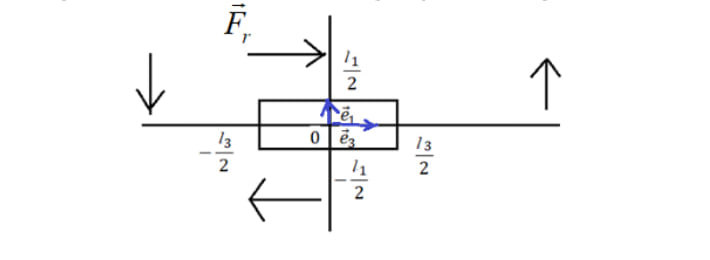
\includegraphics[width=0.7\linewidth]{semester8/img/27}
	\caption{}
	\label{fig:26}
\end{figure}
Тогда для данного цилиндрического тела \( V \) имеет место:
\begin{equation}
\sigma = p \vec{e}_3 = \left( p \delta_{ij} \delta_{j3} \right) \vec{e}_i \otimes \vec{e}_j \quad \label{eq:(264)}
\end{equation}
Т.е. \( \sigma_{ij} = p \delta_{ij} \delta_{j3} \), для всех \( x^i \in V \).
(
$\sigma_{33} = p, \quad \text{остальные} \quad \sigma_{ij} = 0$
)

Поскольку \( p = \text{const} \), то поле напряжений \( \sigma_{ij} \) однородное, т.е. не зависит от \( x_i \). И поле деформаций тоже однородно и имеет вид:
\begin{equation}
\varepsilon = ^4\Pi \cdot\cdot \sigma, \quad \text{т.е.} \quad \varepsilon_{ij} = \Pi _{ijkl} \sigma_{kl} = p \Pi _{ij33} \quad \label{eq:(265)}
\end{equation}
где \( ^4\Pi\) – тензор упругих податливостей.

А перемещение \( \vec{u} \) определяют по формуле Чезаро:
\begin{equation}
\vec{u}(\vec{x}) = \vec{u}_0 + \vec{w}_0 \times (\vec{x} - \vec{x}_0) + \varepsilon \cdot (\vec{x} - \vec{x}_0) \quad \label{eq:(266)}
\end{equation}

\textbf{Доказательство:}

Очевидно, что уравнение равновесия удовлетворяется, если в них подставить \ref{eq:(264)}, так как:
\[
\sigma_{ij,j} = p_{ij} \delta_{i3} \delta_{3j} = p_{i3} \delta_{i3} = 0
\]

Проверяем граничные условия:
\begin{enumerate}
    \item  \( \Sigma_T \): \( \vec{n} \cdot \sigma = \vec{t}_{ne} = 0 \) (на боковой поверхности).

Проверка:
\[
\vec{n} \cdot \sigma|_{\Sigma_T} 
= p \cdot (\vec{n} \cdot \vec{e}_3)_{\Sigma_T} \vec{e}_3 
= \vec{n} \cdot p e_3^2
= \vec{n} \cdot p \vec{e}_3 \otimes \vec{e}_3 
= p \vec{n} \cdot \vec{e}_3 \otimes \vec{e}_3 = 0 \quad \Rightarrow \text{выполнено}.
\]
\item При \( x_3 = \pm L \): \( \vec{n} \cdot \sigma = p \cdot \vec{n} \).

Проверка:
\[
\vec{n} \cdot \sigma|_{\Sigma_3} = p \cdot (\vec{n} \cdot \vec{e}_3)_{\Sigma_3} \vec{e}_3 = p \vec{e}_3 \cdot \vec{e}_3 \otimes \vec{e}_3 = p \vec{e}_3 = p \cdot \vec{n} \quad \Rightarrow \text{выполнено}.
\]
\end{enumerate}

\textbf{Замечание 1.} Поле перемещений \( \vec{u}(\vec{x}) \) по \ref{eq:(264)} определяется неоднозначно – с точностью до \( \vec{u}_0, \vec{w}_0 \) соответствующей точки \( \vec{x}_0 \). Для устранения неоднозначности необходимо дополнительно задать:
\begin{equation}
\vec{u} = \vec{u}_0, \quad \text{для} \quad \vec{x} = \vec{x}_0 \in V \cup \Sigma \quad \label{eq:(267)}
\end{equation}
и
\begin{equation}
\vec{w}_0 = \frac{1}{2} \nabla \times \vec{u}_0, \quad \text{для} \quad \vec{x} = \vec{x}_0 \in V \cup \Sigma \quad \label{eq:(268)}
\end{equation}
\ref{eq:(267)} и \ref{eq:(268)} называют условиями жесткого защемления, если \( \vec{u}_0 = 0, \vec{w}_0 = 0 \). \\В таком случае:

$\vec{u}(\vec{x}) = \varepsilon (\vec{x} - \vec{x}_0) \quad \label{eq:(269)}$


\textbf{Частный случай.}

Граничные условия: вектор напряжений \( \vec{t}_n \) задан на одном торце, а на втором – задана одна продольная компонента вектора перемещений \( u_3 = \text{const} \). Тогда решение задачи линейной теории упругости имеет вид:
\begin{align}
\sigma_{ij} &= p \delta_{i3} \delta_{j3}, \\
\varepsilon_{ij} &= p \Pi_{i j 33} \quad \label{eq:(26*)}\\
u_i &= u_3 \delta_{i3}
\end{align*}
где $u_3 = \varepsilon_{33}(x + L) + u_{3_0}$
\par
Если \( p \equiv\sigma \equiv \frac{F}{S} \) и \( \varepsilon_{33} = \frac{l - l_0}{l_0} \), тогда на основании этого решения:
\begin{equation}
\varepsilon_{33} = \Pi_{3333} \sigma = \frac{1}{E_3} \sigma
\end{equation}
где
\[
F = F \vec{e}_3, \quad l_0 = 2L, \quad S \quad \text{– площадь поверхности, на которую действует сила.}
\]
Из \ref{eq:(26*)} \( \varepsilon_{11} = \frac{l_1 - l_1^0}{l_1^0} \) – поперечная деформация при продольном растяжении и сжатии:
\begin{equation}
\varepsilon_{11} = \Pi_{1133} \sigma = - \frac{\nu_{31}}{E_3} \sigma
\end{equation}

Для ортотропных материалов:
\begin{equation}
\varepsilon_{33} = \Pi_{3333} \sigma = - \frac{1}{E_3} \sigma
\end{equation}
Тогда:
\begin{equation}
\varepsilon_{11} = - \nu_{31} \varepsilon_{33}
\end{equation}

\textbf{Коэффициент Пуассона:}
\begin{equation}
\nu_{31} = - \frac{\varepsilon_{11}}{\varepsilon_{33}}
\end{equation}

Для большинства упругих сред: \( \varepsilon_{33} > 0, \, \varepsilon_{11} < 0, \, \nu_{31} > 0 \).